\documentclass[11pt,oneside,openany]{article}

\usepackage{graphicx}
\usepackage{color}    % to define macros for colors
\usepackage{listings} % package to include source code

\author{Matteo Franchin}

\title{Multiphysics~simulations of magnetic~nanostructures}

%TYPESETTING:----------------------------------------------------------

% Reset page margins properly for doublesided pages

% No headings
\pagestyle{plain}

% 1.5 interline spacing --> corresponds to linespread 1.3
% 2.0 interline spacing --> corresponds to linespread 1.6
\linespread{1.3}

\setlength{\marginparwidth}{0mm}
\setlength{\marginparsep}{0mm}
\setlength{\oddsidemargin}{0.7in} % corresponds to 1 + 0.7 = 1.7 inches
\setlength{\evensidemargin}{0.7in} % corresponds to 1.7 inches
\setlength{\textwidth}{145mm}
\setlength{\textheight}{220mm}
\setlength{\voffset}{-20mm}
\raggedbottom

%----------------------------------------------------------------------
% Extra colors

\definecolor{lightgrey}{cmyk}{0.05,0.05,0.05,0}
\definecolor{gray}{rgb}{0.5,0.5,0.5}

%----------------------------------------------------------------------
% Style for code listings

\lstdefinestyle{defaultstyle}{}
\lstset{language=Python}
\lstset{basicstyle=\ttfamily\scriptsize}
\lstset{showstringspaces=false}
\lstset{keywordstyle=\color{blue}}
\lstset{stringstyle=\color{red}}
\lstset{commentstyle=\color{gray}\emph}
\lstset{numbers=left,frame=single}
\lstset{backgroundcolor=\color{lightgrey}}

\newcommand{\vecs}[2]{\mathbf{#1_{\mathrm{#2}}}}

\begin{document}

\titlepage

\section{Applied field continuously varying in time with Nmag}
In this document we explain how to use Nmag to create a simulation where
the applied field changes continuously with time.
This is an undocumented feature, which can be used, but for which a clean
user interface has not been defined, yet.
Defining a field which changes continuously in time can be useful for many
purposes: applying a pulse with optimal time dependency to excite spin waves
inside a system (with a well controlled window of frequencies) or extending
Nmag by adding an extra term to the applied field.
In this document we will show and explain one example which was used
in the course of the DYNAMAG project to compute the susceptibility
of a disk (spin waves where excited for a defined window of frequencies).
In this example, it is important to apply an homogeneous (in space) magnetic
field with a time dependecy which goes as
$\mathrm{sinc} \, \omega_{\mathrm{max}} t$,
as this allows exciting spin waves with freqencies from 0 to
$\omega_{\mathrm{max}}$.


\subsection{Example: dynamics of a disk excited by a sinc pulse}
In this example we consider a disk. We create the mesh using Netgen and
the following geometry specification file:
%
\lstinputlisting{disk.geo}
%
The resulting mesh is shown in Fig. \ref{fig:mesh}.
%
\begin{figure}[h]
\begin{center}
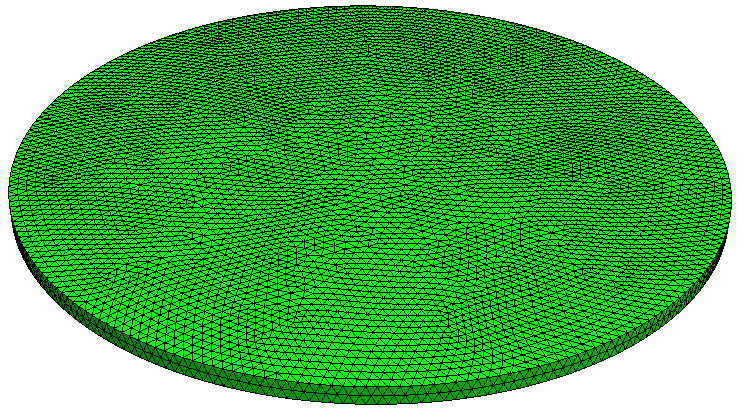
\includegraphics[width=10.0cm]{disk}
\caption[Sketch]{A picture of the mesh used in the simulation.}
\label{fig:mesh}
\end{center}
\end{figure}
%
The simulation script is split in the two figures Fig. \ref{fig:script1of2} and
\ref{fig:script2of2}.  The script can be used to perform two simulations: if
the script is ran for the first time, it just perform a relaxation and saves
the relaxed magnetisation to a file with name \verb|relaxed.h5|. If the script
is ran for a second time, it checks whether this file exist, it finds it, and
loads the initial magnetisation from it. It then applies a pulsed magnetic
field and records the dynamics to disk.

We will now describe the script line-by-line:

\textbf{Lines 1-6:} these are the usual import statements, which often occur
in Nmag scripts. A number of units are also defined: \verb|ps|
for picoseconds, \verb|Hz| for Hertz, etc.

\textbf{Lines 7-10:} these lines define the initial magnetisation used for the
relaxation script (directed towards the positive $x$ axis) and the bias
magnetic field, $\vecs{H}{bias}$, (aligned along the same direction, and with
intensity of 1000 Oersted). $\vecs{H}{bias}$ --- which is uniform in space and
constant in time --- is applied both during relaxation and during the
computation of the dynamics.

\textbf{Lines 11-13:} the stopping dm/dt criterion is set for the relaxation.
This determines how accurate the simulation will be.
The second line defines where the name of the file which will contain the
values of the relaxed magnetisation.

\textbf{Lines 14-20:} these lines define the characteristing of the pulse which
will be applied to the disc (only during the dynamics simulation) in order to
excite spin waves inside it.  The pulse is realised by adding an extra time
dependent field to the bias magnetic field. In other words, the applied field,
$\vecs{H}{app}$, in the dynamics simulation is
$\vecs{H}{app}(t) = \vecs{H}{bias} + \vecs{H}{pulse}(t)$,
and $\vecs{H}{pulse}(t) = H_0 \, \mathrm{sinc}\,\omega (t - t_0)$.
Applying a continuous sinc function is required in order to control the
frequency of the spin waves which are excited.

\textbf{Lines 21-44:} the function \verb|setup_simulation| is used to create
the materials, create the simulation object and load the mesh. These operations
are collected together in this function, as they are needed twice: once for the
relaxation simulation and a second time for the dynamics simulation.  Notice,
how the tolerances are set. Controlling all the tolerances is very important in
this kind of simulations, where accuracy can substantially improve the
results. The function \verb|setup_simulation| returns the simulation object, so
it can be further manipulated after the function has been called.

\begin{figure}[!p]
\lstinputlisting[linerange=1-44]{script.py}
\caption{Part 1.}
\label{fig:script1of2}
\end{figure}

\begin{figure}[!p]
\lstinputlisting[linerange=45-92,firstnumber=45]{script.py}
\caption{Part 2.}
\label{fig:script2of2}
\end{figure}

\textbf{Lines 45-55:} here we check whether the file containing the relaxed
magnetisation exists. If it does not exist, then we run the relaxation
simulation, we create the file and exit (the script ends there). If the file
does exist, then we proceed with the dynamics simulation. Notice that the
relaxation is set up by calling the function \verb|setup_simulation| and the
relaxed magnetisation is saved using the method
\verb|Simulation.save_restart_file|.

\textbf{Lines 56-59:} we setup the simulation for the dynamics using again the
function \verb|setup_simulation| and load the initial magnetisation from the
file which was saved at the end of the relaxation simulation.

\textbf{Lines 60-67:} these lines are used to speed-up the process of setting
the external field. First the external field is set in the normal way using the
method \verb|Simulation.set_H_ext|, then the method
\verb|Simulation.get_subfield| is called to retrieve the Numpy array
corresponding to this field. It must be noted here, that the purpose of
these lines is not to set the external field, but rather to get a Numpy
array which is needed later in the function \verb|update_H_ext|. This is
just a trick to set the applied field in the fastest way possible.

\textbf{Lines 68-88:} these are the most interesting lines in the script.
the line:
%
\lstinputlisting[linerange=87-87,firstnumber=87]{script.py}
%
tells to Nmag that the function \verb|update_H_ext| should be called whenever
the RHS of the Landau-Lifshitz equation is computed, just before computing the
effective field (as a sum of exchange, demag, applied field, etc). The function
\verb|update_H_ext| takes the time \verb|t_su| as input (as a number in
simulation units) and updates the applied field according to the value of
\verb|t_su|. Note that the field is set from a Numpy array, \verb|H_value|,
which is computed as a sum of two Numpy arrays: \verb|H_bias_data|, which was
precomputed before, and \verb|t_amp*H_pulse_data| where \verb|t_amp| is a float
value computed as function of \verb|t_su| and \verb|H_pulse_data| is again a
precomputed Numpy array.  The if statement is used to truncate the sinc
function, when the time has exceeded a value for which the amplitude of the
sinc is very small.  Lines 80 to 84 are used to set the field in such a way
that the timestepper is not automatically reinitialised.  There is a final
point to stress: expressing and computing the field in terms of Numpy arrays
allows to greatly speedup the execution of the function \verb|update_H_ext|.

\textbf{Lines 89-91:} The stopping criterion is disabled and the relaxation
is started. The simulation is stopped at time $t = 10240\,\mathrm{ps}$ and
the fields are saved every 10 picoseconds. Notice, that you may want to
replace \verb|save=[('fields'| with \verb|save=['field_m'| to reduce the
size of the output files (as the data is saved very often, it makes sense
to save just the magnetisation, rather than all the fields). 

\end{document}
